% !TEX root = ../main.tex

\section{Experimental Setup}

Evaluating SAARTHI meant answering three separate questions: does the detection
logic work, can it be trusted statistically, and will it actually run on the
hardware we intend to put in a cab? This section walks through the dataset we
built on, the protocol we used to synthesize fatigue signatures that do not
exist in any public corpus, and the cross-validation scheme that keeps the
reported numbers honest.

\subsection{Dataset Characteristics and Preprocessing}
We built the evaluation on a tailored subset of the NTHU Driver Drowsiness
Dataset (NTHU-DDD). Of the candidates we considered, NTHU-DDD came closest to
the messy reality of a machine cab: a dense collection of operator states
recorded under genuinely awkward conditions, with the kind of physiological
variation that laboratory captures tend to iron out. Table
\ref{tab:dataset_census} gives the census of the subset used for training and
validation.

The mess is the point. A perfectly lit lab dataset, with facial landmarks
tracked under ideal conditions, teaches a model very little about shadows,
head-pose swings, sunglasses, or the plain fact that people's faces differ.
NTHU-DDD contains all of these, and that variance is what forces the model to
learn the difference between an ordinary rapid blink and the slower
physiological drift that marks the onset of fatigue.

\begin{table}[htbp]
\centering
\caption{Dataset census. The evaluation drew on a large subset of NTHU-DDD ---
large enough, in our judgement, to support the statistical claims made in
Section VI.}
\label{tab:dataset_census}
\begin{tabular}{lr}
\toprule
\textbf{Metric} & \textbf{Count} \\
\midrule
Total Raw EAR Samples (Frames) & 450,194 \\
Unique Subjects (Operators) & 22 \\
Distinct Lighting Conditions & 4 \\
Distinct Temporal Sequences & 465 \\
\bottomrule
\end{tabular}
\end{table}

\subsubsection{Preprocessing Pipeline}
Before any features were extracted, the raw video stream went through a
cleaning pass deliberately kept simple enough for a low-power edge device to
reproduce. Where facial landmarks dropped out --- a hand passing over the face,
an extreme head turn --- we forward-filled the gap rather than discard the
sequence, preserving temporal continuity. The cleaned stream was then cut into
rolling windows of size $w = 30$, the value fixed by the stability analysis in
Section IV.

\subsection{Synthetic Hazard Injection Protocol}
Here we ran into a problem that anyone working in industrial safety will
recognize: there is no public dataset of labelled fatigue accidents involving
heavy machinery, and there is no ethical way to produce one --- nobody is going
to let a drowsy operator keep driving an excavator for the sake of a label. So
we injected the hazards ourselves, mathematically.

The idea is to take legitimate, alert physiological signals and perturb them
into micro-sleep and deep-fatigue signatures whose magnitude and duration we
control exactly. Want a prolonged eye closure, or an erratic head drop? Dial it
in. The simulation can then model operators at any point along the fatigue
curve, from barely-detectable early drowsiness to the late stage that precedes
an accident.

\subsubsection{Track A Injection: Overt Kinematic Violations}
Track A deals in hazards the machine itself can report: a boom arm pushed past
its safe operating angle, a travel-speed violation mid-slew, a cab tilted
beyond its stability limit. None of this correlates with the operator's
physiology --- the EAR signal stays untouched --- yet each event demands an
immediate, deterministic response.

We simulate three normalised CAN-bus sensor channels:
\begin{itemize}
    \item \textbf{$s_0$: Boom Angle} (threshold $> 0.85$)
    \item \textbf{$s_1$: Travel Speed} (threshold $> 0.90$)
    \item \textbf{$s_2$: Cab Tilt} (threshold $> 0.80$)
\end{itemize}
In normal operation each channel behaves as $s_c \sim
\mathcal{N}(\mu_c^{\text{safe}}, \sigma_c^2)$, with the safe means held a full
three standard deviations below the alarm thresholds; during a violation
event, at least one channel is driven past its limit. Every channel also
carries Gaussian ADC noise ($\sigma_{\text{noise}} = 0.02$) --- the
quantisation artefacts and vibration-induced jitter that a sensor bolted to a
working excavator cannot avoid.

Violations enter at a $5\%$ window-level rate, which works out to roughly two
non-overlapping events per 1{,}000-frame session, each spanning $w = 30$
frames. Detection is deliberately unglamorous: the rule takes the mean sensor
reading across the window and fires if any channel mean clears its threshold.
That $w$-frame averaging is a standard debounce --- it shrugs off
single-sample ADC glitches while still guaranteeing a detection latency of at
most one window.

\subsubsection{Track B Injection: Covert Fatigue Onset}
Testing the XGBoost physiological model called for a subtler adversary: an
operator who sails through every deterministic Track A check while quietly
succumbing to micro-behavioural fatigue. Fatigue episodes of this kind are rare
in continuous industrial work, so we kept the injection rate conservative at
3\%, split as follows:
\begin{itemize}
    \item \textbf{Micro-Sleeps (2\%):} Short but profound eye closures, lasting
    anywhere from 1.0 to 2.5 seconds.
    \item \textbf{Physiological Drift (1\%):} A gradual slowing of the blink
    rate paired with erratic head-pose variation --- the classic early
    signature of drowsiness.
\end{itemize}

The perturbed signal $E_{anom}(t)$ comes from a linear transformation of the
normal baseline EAR signal $E_{norm}(t)$:
\begin{equation}
    E_{anom}(t) = (E_{norm}(t) \cdot k_v) + k_o
\end{equation}
where $k_v$ scales the variance (droopy eyelid dynamics) and $k_o$ is an
additive offset (a sustained drop in baseline eye openness).

Real operators do not simply switch from alert to asleep; they fatigue
progressively, and often try to mask it. To capture that, both parameters are
driven by a perturbation magnitude $\delta \in [0, 1]$:
\begin{align}
    k_v &= 1 - (\delta \cdot \mathcal{U}(0.1, 0.3)) \\
    k_o &= -\delta \cdot \mathcal{U}(0.05, 0.15)
\end{align}
with $\mathcal{U}$ a uniform random distribution. The formulation matters: it
makes the anomalies degrade the way real physiology degrades, rather than
adding white noise and calling it fatigue. A high $\delta$ corresponds to
late-stage drowsiness --- heavy head bobbing, long eye closures --- while a low
$\delta$ gives the faint early onset that is genuinely hard to catch.

Figure \ref{fig:temporal_distribution} shows where the injected anomalies land
in time, over the first twelve sessions of the actual evaluation stream. Two
regimes are visible at once. Micro-sleeps arrive as short, sharp bursts ---
profound EAR depressions that come and go within a couple of seconds --- while
the drift segments stretch out far longer, dragging the baseline downward for
sustained periods. Because every frame touched by a perturbation is labelled
anomalous, this drift coverage is also what produces the high window-level
anomaly rate ($\approx 88.8\%$) that the class-imbalance analysis in
Section~VII has to contend with. The environment the classifier faces is, by
construction, dynamic and non-stationary.

\subsection{Model Configuration and Hyperparameters}

\begin{figure*}[t]
\centering
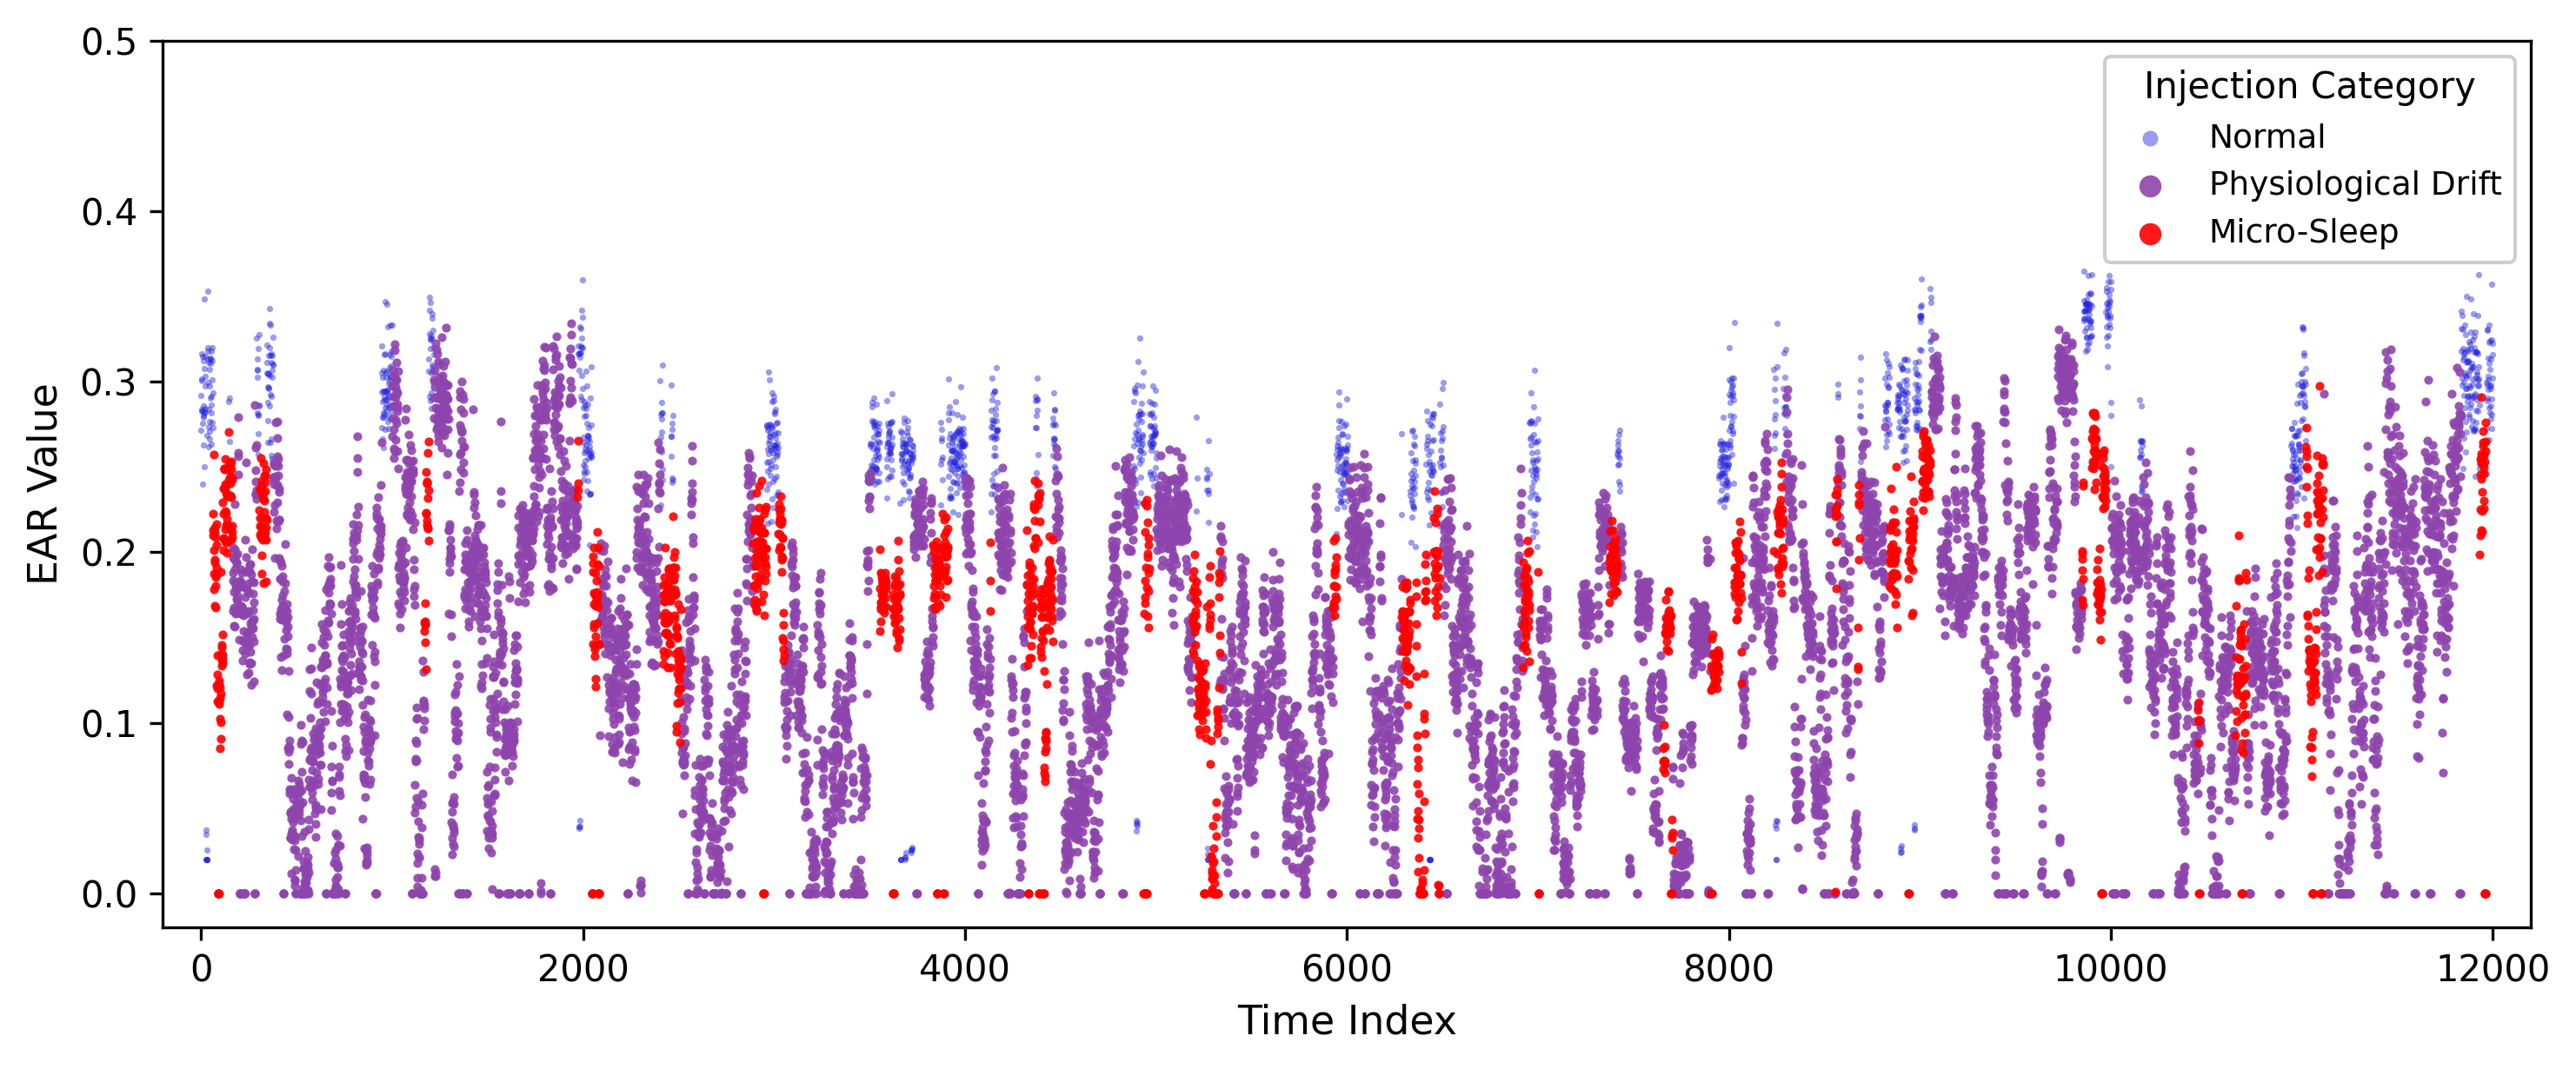
\includegraphics[width=\textwidth]{figures/temporal_distribution.png}
\caption{Temporal distribution of injected hazards over the first twelve
sessions of the evaluation stream (12{,}000 frames, $\delta = 0.5$,
\texttt{SEED=42}). `Micro-Sleep' bursts (red) appear as short, transient EAR
depressions, while `Physiological Drift' segments (purple) suppress the
baseline over sustained stretches; the `Normal' alert baseline (blue) sits
above both. The transient character of the micro-sleep events is why the
$w=30$ sliding window matters: a longer window would smooth these short
bursts out of existence.}
\label{fig:temporal_distribution}
\end{figure*}

We tuned the SAARTHI XGBoost classifier by grid search over a subset of clean,
alert training data. The target was a tight, personalized decision envelope
that still retains the bulk of normal operational samples --- err too far in
either direction and the system becomes either deaf to fatigue or unbearable to
work under. Table \ref{tab:hyperparameters} lists the parameters we settled on.

For the deep learning baselines we used a Denoising Autoencoder (DAE), kept
deliberately small so the comparison stays fair. The network passes the
5-dimensional feature vector through an Encoder
($5 \rightarrow 16 \rightarrow$ Batch Norm (BN) $\rightarrow$ ReLU
$\rightarrow 8$) and a mirrored Decoder
($8 \rightarrow 16 \rightarrow$ BN $\rightarrow$ ReLU $\rightarrow 5$).

\subsubsection{Feature Orthogonality Check}
One question worth settling before training: do the five features actually
carry independent information, or are we feeding the model the same signal five
times? Figure \ref{fig:feature_correlation} shows the feature correlation
matrix.

\begin{figure}[htbp]
\centering
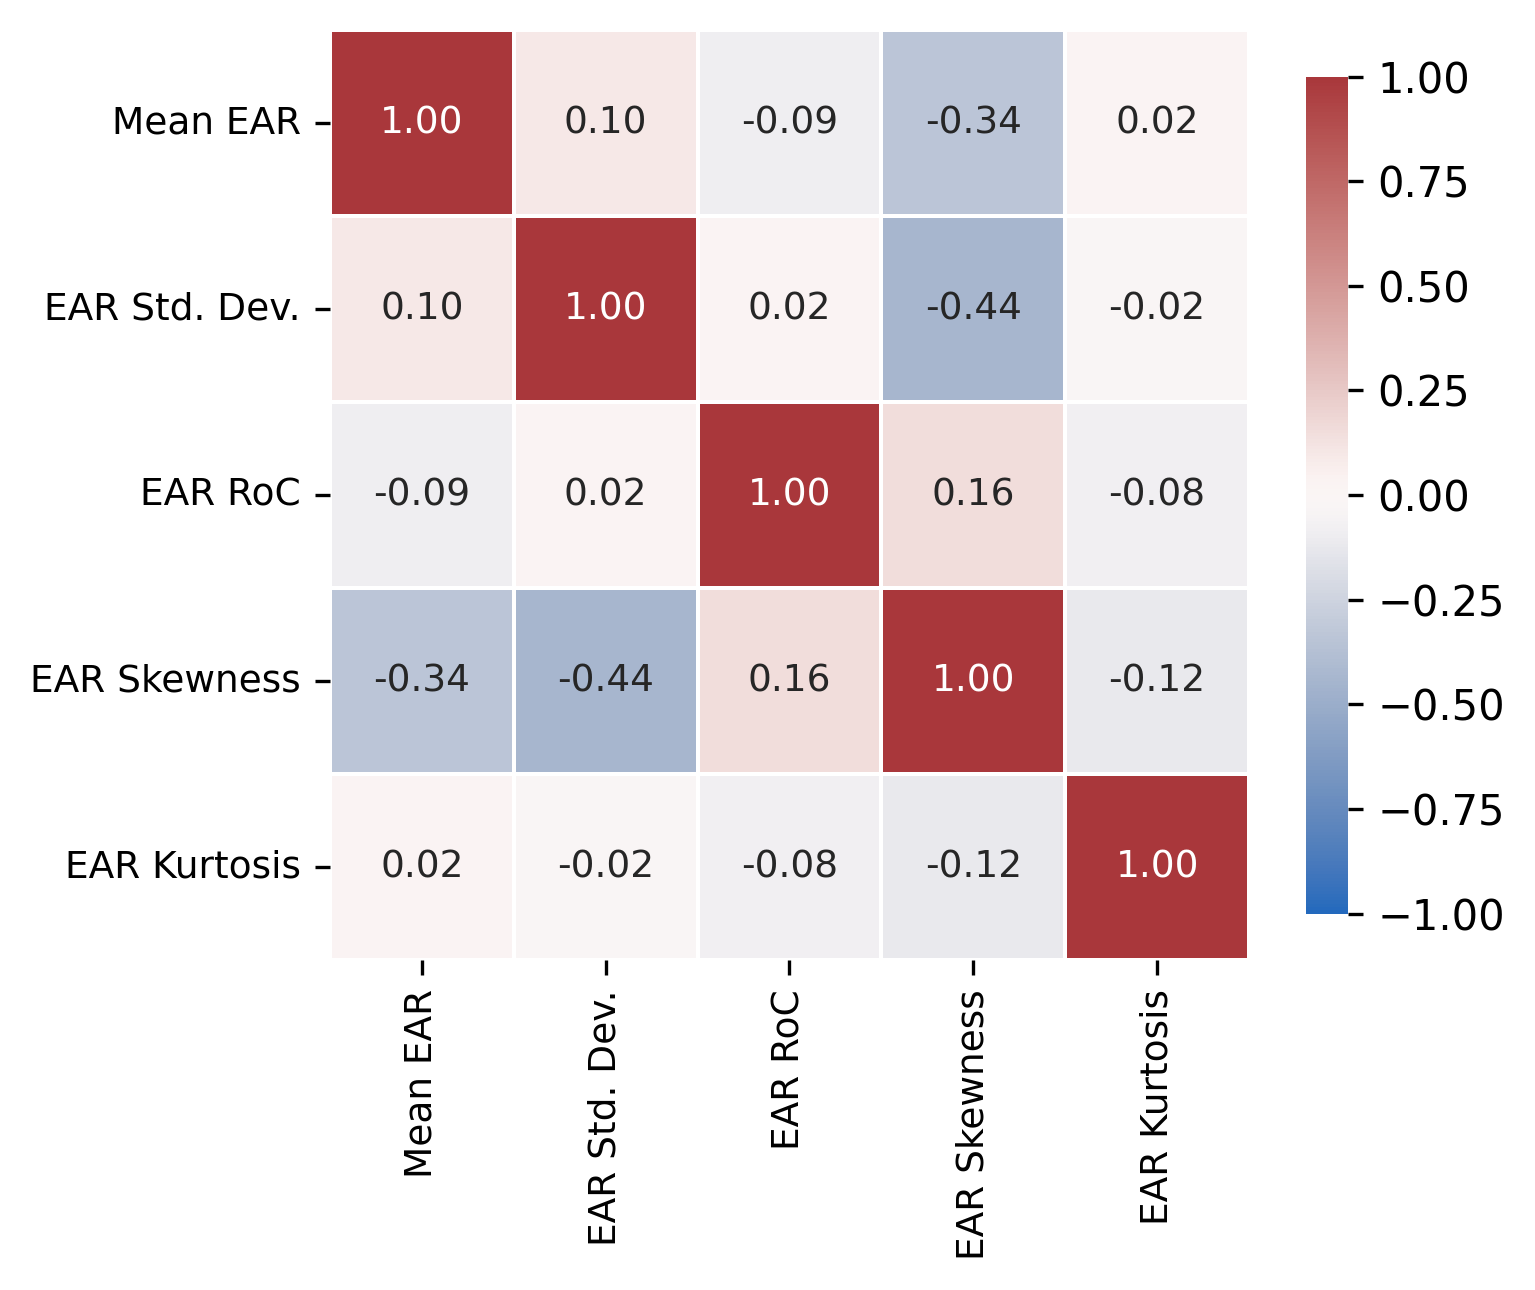
\includegraphics[width=\columnwidth]{figures/feature_correlation.png}
\caption{Feature orthogonality (computed from the full 451{,}515-window
dataset, SEED = 42). The largest off-diagonal correlation is
$r = -0.44$ between Std.\ Dev.\ and Skewness; all remaining pairs
stay below $|r| = 0.35$. No two features carry the same
physiological information.}
\label{fig:feature_correlation}
\end{figure}

To put a number on that independence, we ran a Variance Inflation Factor (VIF)
analysis. The worst offender was Skewness at a VIF of 1.46 --- well within the
acceptable range below the standard trouble threshold of 5.0 (individual VIFs:
Mean EAR 1.14, Std.\ Dev.\ 1.27, $E_{roc}$ 1.04, Skewness 1.46, Kurtosis 1.03).
Each of the five statistical moments therefore contributes its own physiological
evidence to the XGBoost decision boundary rather than restating a neighbour's.

\begin{table}[htbp]
\centering
\caption{Simulation parameters and model configuration. The regularization is
deliberately strict: in a heavy-machinery safety context, a tight physiological
envelope that minimizes False Negatives is worth far more than a forgiving
one.}
\label{tab:hyperparameters}
\begin{tabular}{llp{3.8cm}}
\toprule
\textbf{Category} & \textbf{Parameter} & \textbf{Value / Description} \\
\midrule
\textbf{Dataset} & Source & NTHU-DDD \\
& Window Size ($w$) & 30 samples ($\approx 1.0$ sec) \\
\midrule
\textbf{SAARTHI} & Ensemble Size ($T$) & 100 Trees \\
\textbf{(XGBoost)} & Learning Rate ($\eta$) & 0.1 \\
& Regularization ($\lambda$) & 1.0 (Strict Outlier Tolerance) \\
\midrule
\textbf{Baselines} & Isolation Forest & Contamination=0.05, Trees=100 \\
& Autoencoder & Latent Dim=8, Epochs=50, LR=0.001 \\
\midrule
\textbf{Injection} & Track A Rate & 5\% (Overt Kinematic Hazards) \\
& Track B Rate & 2\% (Micro-Sleeps), 1\% (Physio. Drift) \\
& Perturbation ($\delta$) & Varied $[0.0, 1.0]$ for robustness test \\
\bottomrule
\end{tabular}
\end{table}

\subsection{Hardware Feasibility Benchmarking}
The latency figures reported in Section VI are only as good as their
reproducibility, so all performance benchmarks were run on a single,
standardized compute environment, detailed in Table
\ref{tab:hardware_benchmarks}.

\begin{table}[htbp]
\centering
\caption{Hardware benchmarking environment. All latency and memory figures
were measured directly on the benchmark host using 
\texttt{run\_experiment.py} (SEED = 42).}
\label{tab:hardware_benchmarks}
\begin{tabular}{llp{3.4cm}}
\toprule
\textbf{Category} & \textbf{Component} & \textbf{Specification} \\
\midrule
\textbf{Benchmark} & Processor & Intel Core Ultra 5 125U, 12C/14T @ 3.60 GHz \\
\textbf{Host} & Memory & 15.7 GB RAM \\
& OS & Windows 10 (Build 26200) \\
& Runtime & Python 3.11.9, XGBoost 3.0.2 \\
\midrule
\textbf{Target Edge} & SoC Class & ARM Cortex-A72 (Raspberry Pi 4 / Jetson Nano tier) \\
\textbf{Node} & Memory & 4 GB LPDDR4 \\
& Accelerator & None (CPU-only inference) \\
\midrule
\textbf{Deployed} & Footprint & 165.75 KB (pickle) / 206.79 KB (JSON) \\
\textbf{Model} & Inf.\ Latency & 0.55 ms mean, 0.98 ms p99 \\
\bottomrule
\end{tabular}
\end{table}

The question that actually decides deployment is whether the algorithm survives
on the resource-constrained edge nodes --- Raspberry Pi, the NVIDIA Jetson
series --- that get installed in machinery cabins. Cloud offloading was never an
option; the round-trip latency alone would defeat the purpose. The serialized
XGBoost ensemble occupies 165.75 KB in pickle format (206.79 KB as a portable
JSON booster), measured directly on the benchmark host. Both figures sit well
inside the RAM budget of this hardware class, leaving sufficient headroom for
the concurrent high-frequency video buffer and the CAN bus handlers.

The inference cost is equally manageable. On the benchmark host (Intel Core
Ultra 5 125U), a single 5-feature inference call completes in 0.55 ms on average
($p_{99} = 0.98$ ms). This is two orders of magnitude below the
$T_{\text{human}} \approx 250$ ms human reaction threshold, confirming that
SAARTHI's decision pipeline will never become the bottleneck in the intervention
chain regardless of the edge SoC deployed by the fleet.

\subsection{Validation Methodology}
All results were produced under 10-Fold Stratified Cross-Validation with a
fixed global random seed. Stratification matters here more than usual: hazard
events are rare by construction, and an unstratified split can hand a lazy
classifier an inflated accuracy score simply by starving some folds of
positives. Partitioning so that the Alert-Baseline-to-Fatigued/Hazardous ratio
stays constant across folds closes that loophole. Every metric reported in this
paper is the mean over 10 independent simulation runs.
